\chapter{Background}
\label{cha:introQA}

This chapter offers an overview on some relevant concepts essential to understand the core of this thesis. First we will provide the definition of SAT, MaxSAT and a brief overview of the state-of-the-art algorithms used to efficiently solve them. We will also discuss some extensions of the SAT framework, SMT and OMT, citing some popular solvers built in the last decade to deal with these classes of problem. Lastly, an introduction to quantum computing and the adiabatic quantum annealing is provided.

\section{SAT}
\label{sec:sat}

Computer science problems can be classified according to their computational complexity in returning a solution. Problems that can be solved on a deterministic sequential machine in an amount of time that is polynomial in the size of the input are known as \textbf{P} problems; on the other hand, \textbf{NP} problems do not provide a sub-exponential algorithm capable of determining the existence of a solution. The class of NP problems relevant to our discussion is known as \textbf{Propositional satisfiability problem (SAT)}. \\
SAT definition is quite simple: given a formula made up of Boolean variables as input, our task is to determine if each variable of the input formula can be consistently replaced by the values True ($\top$) or False ($\bot$) so that that the formula evaluates to True. If the condition above can be satisfied, then the Boolean formula is considered \textbf{satisfiable}; on the opposite case, they are defined \textbf{unsatisfiable}. Let's discuss an example: given the following formula involving 2 Boolean variables ($x_1$ and $x_2$):

\begin{equation}
    \varphi = ( x_1 \vee x_2) \wedge (\neg x_1 \vee \neg x_2)
\end{equation}

In this case $\varphi$ is satisfiable: if we set $x_1 = \top$ and $x_2 = \bot$, the entire formula evaluates to True. \\
In order for a Boolean formula to be satisfiable, it is sufficient to obtain a valid assignment: as a result, multiple solutions could be acceptable for a single formula to prove its satisfiability. The problem complexity grows exponentially with the increase of Boolean variables (when $N$ variables are involved, $2^N$ possible assignments have to be tested in the worst case to determine its unsatisfiability), thus its membership to NP. \\
SAT solving found real life applications in HW/SW synthesis and verification problems\cite{satsynth}, cryptography \cite{crypto} and security issues \cite{satsec} and many other tasks. Currently SAT solvers are capable of managing up to $10^6$ variables and $10^7$ disjunctions for some specific cases. On the other hand, more complex problems are actually out of reach despite a low number of variables to manage, in particular related to cryptanalysis and verification of arithmetic circuits. The search of efficiency for these tasks is the ultimate goal of this research. \\
Boolean formulas can be converted to equivalent representations with desired properties than can help SAT solvers in determining its satisfiability. The two most popular Boolean conversions are the \textbf{conjunctive normal form (CNF)} and the \textbf{Tseitin transformation}. \\
A Boolean formula $\varphi$ is written in conjunctive normal form is if it is structured as the conjuction of simpler disjunctive sub-formulas (each disjunction is called clause), satisfying the following formulation:

\begin{equation}
    \bigwedge_{i=1}^L \bigvee_{j_i=1}^{K_i} I_{j_i}
\end{equation}

Each Boolean formula can be reduced to an equivalent CNF formulation applying some transformation rules known as \textbf{De Morgan's rules}:

\begin{equation}
    \neg (\alpha \wedge \beta) = (\neg \alpha \vee \neg \beta)
\end{equation}
\begin{equation}
    \neg (\alpha \vee \beta) = (\neg \alpha \wedge \neg \beta)
\end{equation}

The main issue generated by a CNF conversion is its exponential increase in size; on the contrary the second proposed approach, Tseitin transformation, is capable of simplifying the formula maintaining a linear growth \cite{pa27}. The key idea is the introduction of auxiliary variables to represent the output of subformulas
and then constrain those variables using CNF. In details, given a formula $\varphi$ we need to follow these steps:

\begin{itemize}
    \item We introduce a new variable for each subformula $\psi$ of $\varphi$.
    \item We consider each subformula $\psi = \psi_1 \circ \psi_2$, where $\circ$ can be any Boolean connective, and stipulate representative of $\psi$ is equivalent to representative of $\psi_1 \circ \psi_2$.
    \item Each subformula is converted into its CNF-equivalent formulation.
    \item We can build the Tseitin formula as:
    
    \begin{equation}
        \psi_\varphi \wedge \bigwedge_{\psi_1 \circ \psi_2 \in \textrm{  subf}(\varphi)} \textrm{CNF}(\psi_{\psi_1 \circ \psi_2} = \psi_{\psi_1} \circ \psi_{\psi_2})
    \end{equation}
\end{itemize}

We need to point out how the formula obtained after a Tseitin transformation is not equivalent to its original form (because of the newly introduced variables); despite this, the two Boolean formulas are equisatisfiable, meaning that the first formula is satisfiable whenever the second is and vice versa and thus being suitable to be used for our tasks.

\subsection{How to solve SAT problems: DPLL and CDCL}

The first algorithm acquiring popularity to deal with SAT instances is known as \textbf{Davis–Putnam Logemann–Loveland (DPLL) algorithm} \cite{dpll}. It is a complete, backtracking-based search algorithm for deciding the satisfiability of propositional logic formulae in conjunctive normal form. The solver chooses a literal and assigns a truth value between True and False, opening a new branch; this choice will simplify the formula and the value of a subset of other literals will be bounded. Once no more variable values can be deterministically assigned, we choose a second variable and repeat the procedure described above until we retrieve a satisfying assignment or a conflict is found. In the second case, we perform a chronological backtrack: we jump back to the most-recent open branching point and start the search from that point. If no path reach satisfiability, the formula is considered unsatisfiable. \\
The algorithm described above, albeit working, it quite inefficient because of the amount of resources wasted to perform each backtrack jump. To solve this issue, a variant of the algorithm has been proposed and it is the current state-of-the-art approach implemented in the SAT solvers: \textbf{conflict-driven clause learning (CDCL)} \cite{cdcl}. The algorithm behaviour is similar to DPLL until we reach a conflict: in that case information is collected to efficiently backtrack and avoid lots of redundant search. In particular CDCL relies on: \\

\begin{itemize}
    \item \textbf{Conflict analysis}: once a branch fails, we determine the sub-assignment $\eta$ causing the conflict, determining the conflict clause.
    \item \textbf{Learning}: the conflict clause is stored by the solver into the conflict set, ready to be applied when required.
    \item \textbf{Backjumping}: we can then backtrack to the highest branching point so that the stack contains all-but-one literals in $\eta$, and then unit-propagate the unassigned literal on C.
\end{itemize}

While this approach drastically prunes the search space, we need to take into account the growth of space complexity required to store clauses. Heuristics have been proposed to determine when a learned clause is no more useful for the task in question and can be dropped, limiting the amount of space needed.

\subsection{Representing SAT using And-Inverter Graph}

Each Boolean formula can be represented using different approaches. The structural implementation relevant to the scope of this dissertation is known as \textbf{And-Inverter Graph (AIG)}. An AIG is a directed, acyclic graph characterized by:

\begin{itemize}
    \item Terminal nodes, representing Boolean variables.
    \item Two-input nodes, representing logical conjunctions
    \item Marked edges, representing negation of a logical conjunction.
\end{itemize}

To convert a Boolean problem into an equivalent AIG representation, it is convenient to start from its CNF formulation. From CNF we can trivially construct an AIG by rewriting each OR clause as an AND function using De Morgan’s Law, and then rewriting each AND function with more than 2 inputs as a sequence of 2-input AND functions. An example of AIG representation of a simple Boolean function is shown in Figure 2.1. 

\begin{figure}[t]
	\begin{center}
	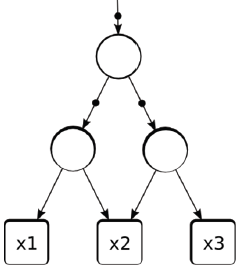
\includegraphics{images/AIG.png}
	\caption{An And-Inverter Graph representing the Boolean formula $\phi = (x_1 \wedge x_2) \vee (x_2 \wedge x_3)$}
	\end{center}
\end{figure}



\section{MaxSAT}
A subclass of SAT problems is called \textbf{weighted maximum satisfiability}, or \textbf{MaxSAT}. A MaxSAT formula can be seen as optimization extension of SAT: the formula is defined as a conjunction of clauses and, for each clause, a weight (a positive real number) is assigned. Given a Boolean assignment of its variables, a score is calculated considering the weights of all satisfied clauses. This addition changes the perspective of the problem: every assignment can now be considered acceptable, since some clauses can be falsified. As a consequence MaxSat defines a new task: find a Boolean assignment so that the associated score is maximum. Similarly to SAT, multiple assignments can be the solution of a MaxSAT instance, resulting in multiple valid assignments. \\
To better understand it, we cover it using an example. We will consider the following Boolean formula:

\begin{equation}
    \varphi = ( x_1 \vee x_2) \wedge (\neg x_1 \vee \neg x_2) \wedge ( x_1 \vee \neg x_2) \wedge (\neg x_1 \vee x_2)
\end{equation}

Each clause has also an additional weight: first clause from left has a score of 1, each subsequent clause's weight is higher by 1 with respect to the precedent. Clearly no assignment could satisfy all clauses at the same time, but this has no interest since we are solving a MaxSAT problem. Quickly considering all possible assignments, we can state that the one guaranteeing the maximum total score is $x_1 = \bot$ and $x_2 = \bot$, satisfying respectively the clauses with weights 2, 3 and 4. No other Boolean assignment could achieve the same result, so this is the only solution to our MaxSAT problem.

\section{Satisfiability Modulo Theories}

Satisfiability Modulo Theories represents an extension to the SAT problem. The input and the final goal remain the same as SAT: this means that we have to deal with first-order logic formulas and we search for a valid assignment of variables satisfying such formulas. The main difference relies on the fact that binary boolean variables can be replaced by predicates and functions belonging to non-binary theories. Some of the most relevant theories in the Formal Verification fields are:

\begin{itemize}
    \item Linear Arithmetic over Integers, Real or both (LIRA)
    \item Bit vector arithmetic (BV)
    \item Floating-point arithmetic(FP)
    \item Uninterpreted functions (UF)
\end{itemize}

Given the non-binary nature of these theories, novel approaches have been studied and tested to efficiently evaluate the satisfiability of a given formula. At the current state, the most widely used algorithm is known as \textbf{Lazy SMT solving}\cite{lazysmt}, whose core idea will be briefly explained to the reader for a better comprehension. Given an SMT formula and a subset of theories, we produce a Boolean abstraction formula in which each non-binary predicate is replaced by a binary variable. This new formula is then fed to a CDCL SAT solver and used to search a satisfiable assignment. When a satisfiable assignment is obtained, the corresponding set of T-literals that make up the original problem are fed to specialized theory solvers. If each clause if T-consistent, then we proved the satisfibility of the original formula; otherwise, the conflict clauses causing unsatisfiability are extracted and learned by the CDCL algorithm , permitting the evaluation of new assignments. The algorithm goes on until satisfiability is proved or no more assignment can be returned, proving its unsatisfiability. \\
In order to be evaluated, the instance of a SMT problem has to be instantiated using a standard format. Regarding SMT encoding, SMT-LIB is the international initiative on top of which most SMT solvers are built. SMT-LIB does not only promote common input and output languages for SMT solvers; it also provides standard rigorous descriptions of background theories used in SMT systems and establishes benchmarks that can be used to test the solvers to highlight weaknesses and strengths. \\
The syntax of SMT-LIB-based tools is quite simple. First, we define properties of the problem and solver options (for instance determine if we want to extract unsat cores). We can also set a theory, so that efficient algorithms and heuristics are applied during execution to improve performances. After this introduction, we declare constants, variables and functions. Then assertions are expressed: they bind the values of variables, restricting the range of satisfying solutions. A simple example is provided in listing 2.1. \\
\begin{lstlisting}[style=interfaces,caption=An example of SMT-LIB encoding.]
(set-info :smt-lib-version 2.6)
(set-option :print-success false)
(set-option :produce-models true)

(declare-const x Int)
(declare-const y Int)
(declare-fun f (Int) Int)

(assert (= (f x) (f y)))
(assert (not (= x y)))

(check-sat)
(get-value (x y))
\end{lstlisting}
Among the solvers accepting SMT-LIB as input format, University of Trento and the Bruno Kessler Foundation have developed a SMT solver, called MathSAT \cite{pa16}. The code, written in C++, support all the theories mentioned above, plus other logics as Arrays arithmetic. It also supports interesting functionalities such as generation of models and proofs for satisfiable problem, extraction of unsatisfiable cores for the unsatisfiable ones and incrementality.

\section{Optimization Modulo Theories}

Optimization Modulo Theories represents an extension to the SMT framework. In addition to the already described first-order formulas involving non-binary logics, we focus on defining one or more non-binary objective function. As a result, retrieving a satisfying assignment is not sufficient anymore: the goal is now obtaining a valid model while minimizing/maximizing the objective functions, according to our choice.\\
The language used to encode OMT problems is an extension of the SMT-LIB standards. In addition to the syntax already discussed for SMT-LIB, some commands are available to define the cost functions we desire to optimize and the direction of optimization. The structure of this command is:

\begin{equation*}
    \textbf{solve [maximize/minimize] $<$cost function$>$}
\end{equation*}

If permitted by the solver, we can also write multi-objective optimization problems. multi-objective optimization problems  require the presence of some instructions to determine the philosophy adopted to determine the goodness of a solution. Example of valid approaches are:

\begin{itemize}
    \item \textbf{Pareto Optimality}: given two different solutions and a set of $n$ cost functions $x_1...x_n$, we state that the first solution is better to the second one according to this criterion if there exists a cost function $x_i$ (where $1\leq i\leq n$) so that $x_i$ calculated on the values of the first solution dominates the value obtained using the second solution; in addition to that, for each cost function $x_i$ the first solution obtain better or equal values than the second one. When using this criterion, multiple solutions can satisfy these conditions: the set of these valid assignment is called \textbf{Pareto front}.
    \item \textbf{Lexicographic Optimality}: first we define a total order among the various cost functions, determining  a hierarchy. Given two different solutions, we will first compare the value of the first cost function on this hierarchy for both of them; if one of these solutions dominates the other it is chosen as optimal, otherwise we will compare the value associated to the second cost function and so on until reaching the last one.
\end{itemize}

The jointly work between FBK and University of Trento gave birth to an Optimization Modulo Theories solver, \textit{OptiMathSAT} \cite{pa25}*.

\section{Constraint Programming and MiniZinc}

Constraint Programming is an alternative paradigm for solving combinatorial problems. A Constraint Satisfaction Problem (CSP) is defined by a set of variables, each one with its domain of values, and a number of constraints, relations among a subset of the variables. A simple example of constraint is called ALLDIFFERENT: given some variables as input to this relation, it ensure no involved variable will assume the same value. The usual output of a CSP is a a valid assignment for each declared variables, if possible. The CSP has been extended to deal with the search of optimal solution with respect to some objective function, similarly to what happened to SMT: these problem are referred as Constraint Optimization Problems (COP).
Due to the large amount of constraint available and its representational power, Constraint Programming popularity is growing in the last years and it is actually used in some formal verification related tasks. \\
MiniZinc is the most popular high-level declarative language used to encode both CSP and COP instances. It is developed at Monash University in collaboration with Data61 Decision Sciences and the University of Melbourne. Each MiniZinc model first declares each variable needed to define the problem; optionally a value can be assigned, obtaining a parameter whose behaviour is similar to constants. Variables which are not initialized are known as decision variable and their value is determined by the solver, trying to satisfying the conditions that will follow. The next component of the model are the constraints, Boolean expression defining bounds to the value each decision variable can assume. Lastly we have a line expressing if we are working with CSP (so we only focus on knowing if there exists an assignment satisfying each variable domain and making true all constrains) or COP (in this case the user has to define the objective function to optimize and the direction of optimization). A simple example is provided in listing 1.2.

\begin{lstlisting}[style=interfaces,caption=An example of MiniZinc encoding regarding the popular Stable Marriage Problem.]
int: n;
enum Man = anon_enum(n);
enum Woman = anon_enum(n);
array[Woman, Man] of int: rankWomen;
array[Man, Woman] of int: rankMen;
array[Man] of var Woman: wife;
array[Woman] of var Man: husband;

constraint forall (m in Man) (husband[wife[m]]=m);
constraint forall (w in Woman) (wife[husband[w]]=w);
constraint forall (m in Man, o in Woman) (
     rankMen[m,o] < rankMen[m,wife[m]] -> 
         rankWomen[o,husband[o]] < rankWomen[o,m] );
constraint forall (w in Woman, o in Man) (
     rankWomen[w,o] < rankWomen[w,husband[w]] -> 
         rankMen[o,wife[o]] < rankMen[o,w] );
solve satisfy;
\end{lstlisting}

\subsection{Bridging CP and OMT}

OMT presents some specific affinities that make it a valid candidate to deal with CSP: the availability of decision procedures for infinite-precision arithmetic, the efficient combination of
Boolean and arithmetical reasoning and the ability to produce conflict explanations are shared between the two paradigms and it is not a case both are used to deal with formal verification problems. Achieving this task benefits the progression of the current state-of-the-art: the comparison between OMT solvers and CP tools on problems that do not belong to their original application domain extends their application in novel fields and speed up the process of finding critical points for future research. \\ 
Despite that, transforming a CP instance into a OMT problem is not trivial; in particular there are multiple valid formulation of a CP problem into an OMT instance. Using one option instead of the others requires particular attention, since this choice could drastically affect performances (as shown in []). This situation represents the first issue hardening the bridging task. In addition to this difficulty, there are some MiniZinc features that requires a careful mapping to the SMT-LIB standard. In particular:

\begin{itemize}
    \item FlatZinc support three basic scalar types (int, float and bool) and two compound types (set and array). Compound types do not have a direct correspondence in the SMT-LIB standard; moreover integer and float can be represented using finite precision (using respectively bit-vector and floating point arithmetic) or applying the linear arithmetic theory.
    \item MiniZinc introduced local and global constraints to express complex relations among variables. OMT solver currently do not introduce ad hoc decision procedures to manage them efficiently.
    \item MiniZinc is capable of dealing with non-linear and transcendental functions, such as the logarithm or the cosine function. On the other hand, not every solver built on SMT-LIB support them.
\end{itemize}

\section{Quantum Annealer}
\label{sec:quantum}

In order to achieve efficiency in solving the hardest tasks, one of the proposed techniques involves the exploit of quantum technologies. In the case at issue \textbf{Quantum Annealers (QA)} have been proved to be effective for this task. \\
Quantum annealers are specialized chips that exploit particular quantum effects (such as superposition and tunneling) to sample or minimize energy configurations. Each configuration is composed by binary variables $z_i$ which can assume a value -1 or 1, representing their state. The energy configuration can be represented using the Ising Hamiltonian function, whose structure is the following:

\begin{equation}
    H(\textbf{\underline{z}}) = \sum_{i \in V} h_iz_i + \sum_{\langle i,j\rangle \in E} J_{ij} z_iz_j
\end{equation}

Formula 2.7 shows the parameters that influence the system's behaviour: 

\begin{itemize}
    \item $h_i$ are called \textbf{biases} and are defined as a real number in range $[-2,2]$
    \item $J_{ij}$ and lastly $J_{ij}$ are called \textbf{couplings} to the connected pair of qubits at index $i$ and $j$ and is a real number in range $[-1,1]$.
\end{itemize}

The search of the ground state of an Ising model is known as \textbf{quadratic unconstrained binary optimization (QUBO)} problem. \\

\subsection{The SQUID transistor}

 The minimal unit composing a quantum annealear is called \textbf{qubit}: a qubit can assume a symbol value of 0, 1 or a superimposition of 0 and 1. The physical devices used to build qubits are the \textbf{Superconducting QUantum Interference Devices (SQUID)}, where the word interference refers to the electrons patterns that give birth to quantum effects. The structure of this qubit transistor is defined by two superconductor coupled by a weak link, usually a thin insulating barrier. Transistors satisfying these conditions are subject to the \textbf{Josephson effect}. The superconducting qubit structure instead encodes 2 states as tiny magnetic fields, which either point up or down. We call these states +1 and -1, and they correspond to the two states that the qubit can 'choose' between. Using the quantum mechanics that is accessible with these structures, we can control this object so that we can put the qubit into a superposition of these two states as described earlier. So by adjusting a control knob on the quantum computer, you can put all the qubits into a superposition state where it hasn't yet decided which of those +1, -1 states to be. The behavior of quantum computers lie in between deterministic
and non-deterministic machines, more powerful than deterministic, but bound by quantum-mechanic laws to less than the vast possibilities of non-deterministic automata \cite{pa11}.\\
  Each ring can be superimposed to other rings, defining more complex architectures and admitting an exchange of information among different qubits (thus the definition of couplings in the Ising formula). Figure 2.2 shows the physical structure of a qubit.\\
  
  \begin{figure}[t]
	\begin{center}
	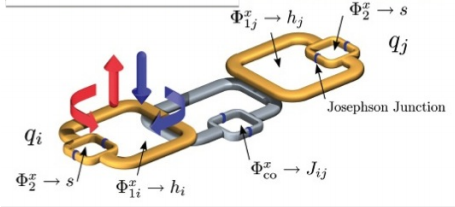
\includegraphics{images/QA.PNG}
	\caption{A physical representation of qubits in an Quantum Annealer.}
	\end{center}
\end{figure}

\subsection{D-Wave Quantum Annealers}

The entire energy configuration can be represented as a connected graph, where vertexes represent our qubits and edges represent connections between qubits. This configuration highlights how qubits' ground state is not considered independently, but their interaction with neighbour qubits alters the final energy state of our configuration. The choice of a specific quantum annealer influences the formulation of an Ising model: each annealer has a specific architecture and specific properties, constraining the formulation of a problem. In this thesis we will concentrate on annealers developed by the Canadian company D-Wave \cite{Dwave}. In the beginning, the Canadian company aimed in increasing the number of available qubits, obtaining Moore-like growth as shown in figure 2.3. 
\begin{figure}[t]
	\begin{center}
	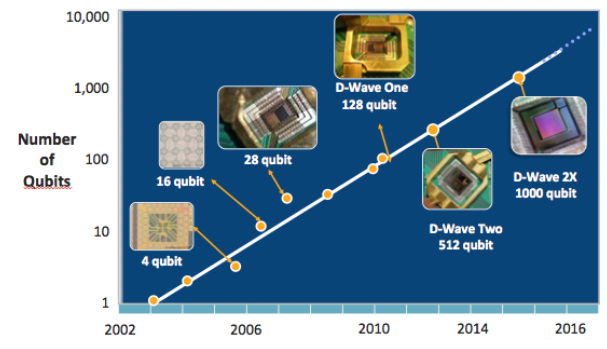
\includegraphics{images/DwaveMoore.PNG}
	\caption{D-Wave annealers growth over the years. Courtesy of D-Wave Systems Inc.}
	\end{center}
\end{figure}
In a second phase, the company put its effort in defining novel structures with better connections and fewer wasted qubits. Currently D-Wave has already developed and produced a first quantum system, known as \textbf{Chimera}. The basic features of this architecture are:

\begin{itemize}
    \item The basic unit is the tile, which contains 8 qubits.
    \item Qubits of a cell unit are grouped into two groups (the horizontal and vertical qubits): qubits belonging to the same group are connected to qubits of the opposite group thanks to couplings.
    \item Unit cells are tiled vertically and horizontally with adjacent qubits connected, creating a 16 $\times$ 16 lattice of 2048 qubits.
    \item From previous constraints, we can see how each qubits can be connected to a maximum of 6 other variables, resulting in the sparsity of the adjacency matrix. Qubits that are not connected to each other are managed setting the related coupling value to 0.
\end{itemize}

In addition to this structure, D-Wave is already studying new architectures overcoming the sparsity of the graph and the absence of cliques; in 2019 the company proposed a new architecture called \textbf{Pegasus}. The properties of this system are:

\begin{itemize}
    \item The number of qubits is $24*N*(N-1)$, where $N$ is an integer number.
    \item The architecture is less modular than Chimera and, in particular, it is not structured in 8-qubit tiles.
    \item Pegasus graph is less sparse than Chimera, presenting an higher number of interleavings among qubits (exactly 15 couplings for a single qubit).
    \item The increasing number of couplings have given the opportunity to obtain huge progress with respect to the old model. In particular, Pegasus provides 3 and 4-cliques and qubit duplication.
\end{itemize}

Figure 2.4 shows the graphs representing both Chimera and Pegasus topologies, rapidly displaying the main differences between the two models. 

\begin{figure}
\centering
\begin{subfigure}[b]{0.55\textwidth}
   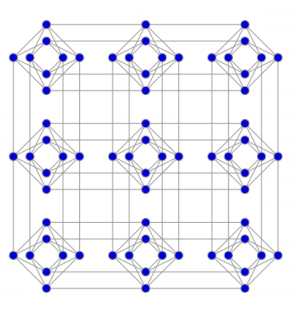
\includegraphics[width=1\linewidth]{images/QATile.PNG}
   \caption{}
   \label{fig:Ng1} 
\end{subfigure}

\begin{subfigure}[b]{0.55\textwidth}
   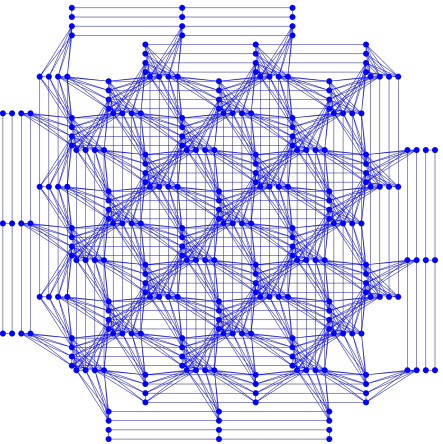
\includegraphics[width=1\linewidth]{images/Pegas.PNG}
   \caption{}
   \label{fig:Ng2}
\end{subfigure}
\caption{A representation of the two architecture proposed by D-Wave, respectively: (a) $3*3$ tiles sub-graph of Chimera (b) the graph of Pegasus6.}
\end{figure}

\newpage

